% !TEX TS-program = xelatex
\documentclass[12pt]{article}
% Margins adjusted slightly for density, can be reverted to 1in if preferred
\usepackage[a4paper,margin=0.8in]{geometry} 
\usepackage{graphicx}
\usepackage[rgb]{xcolor} % Use rgb model for defined colors
\usepackage{fontspec}
\usepackage{tikz}
\usetikzlibrary{positioning, shapes.geometric, arrows.meta, shadows.blur} % Added arrows.meta and shapes
\usepackage[skins,breakable]{tcolorbox} % Added breakable for boxes potentially spanning columns/pages
\usepackage{titlesec}
\usepackage{array} % For >{\bfseries} and p{width} columns
\usepackage{caption} % Although not using standard \caption, load for potential future use/compatibility
\usepackage{multicol}
\usepackage{booktabs} % Professional tables
\usepackage{tabularx} % For dense horizontal packing rules (\toprule, \midrule, \bottomrule)
\usepackage{longtable} % Potentially needed for roadmap, though spanning columns might be better
\usepackage{enumitem} % For customizing lists if needed
\usepackage{ragged2e} % For potentially better justification in columns (\RaggedRight)
\usepackage[final]{microtype} % Improves typography

% --- Custom Colors ---
\definecolor{axiorMagenta}{RGB}{180, 44, 120} % Modern magenta variant
\definecolor{axiorMagentaLight}{RGB}{245, 220, 235}
\definecolor{axiorGray}{RGB}{245, 245, 250}

% --- Stylish Fonts ---
\setmainfont{Arial} % Main body font
\newfontfamily\brochuretitle{Arial} % Font for main titles/headers
\newfontfamily\brochuresubtitle{Arial} % Font for subtitles/secondary headers (fallback for compatibility)

% --- Section Title Formatting ---
% Using '*' versions for unnumbered sections, common in brochures
\titleformat{\section}{\brochuretitle\Huge\bfseries\color{axiorMagenta}}{}{0em}{}
\titleformat{\subsection}{\brochuresubtitle\LARGE\bfseries\color{axiorMagenta}}{}{0em}{\vspace{0.5em}} % Added spacing before subsection

% --- Custom TColorBox Styles ---
% Highlight box for key messages/quotes (light magenta background, dark magenta frame)
\newtcolorbox{highlightbox}[1][]{
  colback=axiorMagentaLight,
  colframe=axiorMagenta,
  boxrule=1pt,
  arc=4pt,
  fonttitle=\bfseries,
  coltitle=black,
  attach boxed title to top left={yshift=-0.1in,xshift=0.15in},
  boxed title style={colback=white,arc=2pt,outer arc=2pt},
  breakable, % Allow box to break across columns/pages
  left=4pt, right=4pt, top=4pt, bottom=4pt, % Internal padding
  #1 % Allow additional options
}

% Infobox for technical details or sidebars (gray background, thin magenta border)
\newtcolorbox{infobox}[1][]{
  colback=axiorGray,
  colframe=axiorMagenta,
  boxrule=0.5pt, % Thinner rule
  arc=2pt,
  fonttitle=\bfseries\brochuresubtitle\color{axiorMagenta}, % Subtitle font for title
  breakable,
  left=4pt, right=4pt, top=4pt, bottom=4pt,
  #1
}

% Sidebar box for small notes (very light background, no frame)
\newtcolorbox{sidebar}[1][]{
  colback=axiorGray!50, % Lighter gray
  colframe=white, % No visible frame
  boxrule=0pt,
  arc=0pt,
  fontupper=\footnotesize, % Smaller font for sidebars
  breakable,
  left=3pt, right=3pt, top=3pt, bottom=3pt,
  #1
}

% --- Helper Commands ---
\newcommand{\placeholder}[1]{
  \begin{tikzpicture}
    \node[draw=gray, dashed, text width=0.9\linewidth, align=center, minimum height=2cm] 
    {\footnotesize\textcolor{gray}{Placeholder for: #1}};
  \end{tikzpicture}
}

% --- Document Start ---
\begin{document}
\setcounter{secnumdepth}{0} % Suppress section numbering for brochure style
\pagestyle{plain} % Keep page numbers for now

% ======================================================================
% PAGE 1: THE GRAND SYNTHESIS & THE STACK
% ======================================================================
\begin{center}
    {\brochuretitle\Huge\bfseries\color{axiorMagenta} The Grand Synthesis: AI Infrastructure for the Age of Agency}
\end{center}
\vspace{1em}

% --- Densely packed Vision & Context and Why Now? using tabularx ---
\begin{tabularx}{\textwidth}{@{}X X@{}}
\textbf{\large Vision \& Context}\newline
Axior is a chipmaker on a mission to shatter the monopoly of San Francisco AI hardware giants. We are creating a “DeepSeek moment” for the hardware layer. We achieve this by delivering open, modular, and accessible AI chips and modules that empower developers, researchers, and businesses to build, scale, and own their AI inference infrastructure, without vendor lock-in.

Our platform is designed for the new wave of local and edge AI, where privacy, cost, and flexibility matter most.

\scriptsize\textbf{Why Inference?} --- All innovation is bottlenecked by closed, cloud-centric hardware. Local inference enables privacy, low-latency, and cost-effective deployment. This empowers escape from the data-scavenging status quo to mission-driven models \& organizations. While AI training remains a crucial part of most ML advances, it is still largely confined to massive datacenters due to its immense compute requirements. But the future is on the inference side, where models run on end-user devices, not just in the cloud. For many edges of the agentic era, inference matters critically. Unlocking the AI edge, then, is not just a technical feat---it’s a lever of the movement and competitive wave of the agency. This shift unleashes the next wave of innovation and compels a new subset of power-users, by empowering a frontier of otherwise consumers to become the transformative providers.
&
\textbf{\large Why Now? The Rise of Local AI Clusters}\newline
\scriptsize Mac Mini clusters are already being used for local AI inference, but they are closed, expensive, and not modular. Unified memory and efficient SoCs have reinvented workstations (AppleSilicon), but those solutions are expensive, closed, and not modular. The edge AI hardware market is projected to more than double by 2028, with demand for local, private, and accessible inference networks. No efficient competitors offer open, modular, jettison-compatible SoMs with unified DDR5 memory and clustering support.
\end{tabularx}

% --- Resume two-column layout for the rest of the page ---
\begin{multicols}{2}

\section{\color{axiorMagenta} The Four Pillars}

\textbf{Axior:} Axior is building the “Raspberry Pi of AI,” the foundation for the next generation of open, accessible, and scalable AI hardware, to power the new wave of local AI innovation. Our platform is designed for DIY AI enthusiasts, consumer devices, and AI application developers needing scalable, open, and affordable inference.

\vspace{0.7em}

\textbf{Lattice:} Lattice is an open protocol and runtime for mesh, agentic AI, enabling anyone, anywhere, to contribute compute and co-create resilient, intelligent systems beyond the limits of the cloud. At its core, Lattice is a self-organizing, peer-to-peer protocol and runtime for agentic AI workloads.

\vspace{0.7em}

\textbf{SOUL:} SOUL is a modular, extensible Python framework for developing meta-agents, “Soulmades,” characterized by inducing purposeful agency, distinct perspectives, and the ability to act based on an internal agenda into generic agents. It moves beyond reactive, text-wall generating models towards AI that exhibits “specific and objective” understanding.

\vspace{0.7em}

\textbf{vhybZ:} vhybZ is a new kind of platform where anyone can co-create dynamic, multimodal digital experiences alongside AI, going far beyond chatbot text walls or static apps. vhybZ is where human creativity and agentic intelligence merge, a true “humagentic” society.

\vspace{1em}

% Optional Visual for Page 1 - Currently omitted as per strict adherence to prompt V2 which didn't require stack diagram or Ai1 render here.
% Could add Ai1 render here if needed for balance:
% \begin{center}
%   
\includegraphics[width=0.8\linewidth]{./assets/Ai1_render.png}
%   \captionof{figure}{\footnotesize Axior Ai1: Open, Modular AI Silicon}
% \end{center}

\end{multicols}


% ======================================================================
% PAGE 2: AXIOR DEEP DIVE
% ======================================================================
\begin{center}
    {\brochuretitle\Huge\bfseries\color{axiorMagenta} Axior Deep Dive: Open, Modular AI Hardware}
\end{center}
\vspace{1em}

\begin{multicols}{2}

% --- Axior Ai1 SoM ---
\subsection{Axior Ai1 SoM}
\begin{center}
\begin{tabular}{@{} >{\bfseries}l p{0.55\linewidth} @{}} % Adjusted column width
\toprule
\textbf{Feature}      & \textbf{Specification} \\
\midrule
Form Factor  & Extended Jetson NX (70 × 45 mm, 4 SODIMM slots) \\
Connector    & 260-pin SO-DIMM (Jetson-compatible) \\
Memory       & 4× DDR5 SODIMM (vertical, 1 per channel) \\
Max RAM      & 128GB/slot today (512GB total); future 1TB+ \\
I/O          & PCIe Gen4×4, USB 3.2×2, HDMI/DP++, 2× MIPI-CSI, GbE/10GbE, SDIO, GPIO/I²C/SPI/UART \\
Clustering   & Carrier boards: 1–4 SoMs, PCIe/10GbE mesh \\
Power        & 5–12V input, on-module PMIC \\
Thermal      & Copper slug, vapor spreader, optional blower \\
\bottomrule
\end{tabular}
\end{center}
\vspace{0.5em}
\small Jetson carrier compatibility: Full pinout, drop-in for Jetson NX ecosystem. Unified memory: CPU, GPU, NPU share DDR5 for large LLMs, vision, and audio. Modular RAM: SODIMM unlocks affordable upgrades and future capacity.

\vspace{1em} % Spacing

% --- Axior Ai1 SoC ---
\subsection{Axior Ai1 SoC}
\begin{center}
\begin{tabular}{@{} >{\bfseries}l p{0.35\linewidth} p{0.45\linewidth} @{}} % Adjusted widths
\toprule
\textbf{Subsystem}   & \textbf{IP Core / Vendor}           & \textbf{Features / Differentiators} \\
\midrule
CPU         & 8× Cortex-A78AE (Arm)     & ECC, ASIL-D, high-perf Linux, 2.2GHz \\
GPU         & PowerVR BXE-BX4-64        & Vulkan 1.3, OpenCL 3.1, 64 clusters \\
NPU         & 4× Flex Logix InferX X1   & 40+ TOPS INT8, modular, ONNX/vLLM/TVM support \\
DSP         & Cadence HiFi 5            & Voice/audio acceleration \\
Memory Ctrl & Synopsys DDR5 4-ch + PHY  & 4× SODIMM, up to 512GB, ECC, future 1TB+ \\
PCIe        & Gen4 ×4                   & Scalable clustering, NVMe/10GbE/expansion \\
NoC         & FlexNoC 5 (Arteris)       & 512-bit coherent interconnect \\
Security    & Arm TrustZone, CryptoCell-312, TPM & Secure boot, eFuse OTP, Infineon SLB9670 TPM \\
PMIC        & Dialog DA9063-L or Renesas RAA215300 & Multi-rail, DDR5 VPP, sequencing \\
Process     & TSMC N7/N6 (130–140 mm² die) & Low power: ~3W idle, 18–25W peak \\
\bottomrule
\end{tabular}
\end{center}
\vspace{0.5em}
\small Estimated SoC retail cost: \$30–40 (assuming ~100K internal production volume). Entry-tier: \$149–179 for Ai1 SoM with 32GB DDR5 unified memory (usable by AI models). Scales to \$199–249 with 64GB modules or higher. Modular RAM: Users can plug in off-the-shelf DDR5, this is our unique differentiator.

\vspace{1em}

% --- Go-to-Market \& Use Cases ---
\subsection{Go-to-Market \& Use Cases}
Axior’s initial focus is on empowering developers, researchers, and startups who require affordable, scalable, and private AI inference at the edge. Early use cases include:
\begin{itemize}[leftmargin=*, itemsep=0pt, topsep=2pt]
    \item Local AI clusters for research labs and universities
    \item Smart device manufacturers seeking on-device intelligence
    \item Privacy-first applications in healthcare, robotics, and IoT
    \item AI hobbyists and makers building custom solutions
\end{itemize}
\vspace{0.3em}
Our modular approach allows rapid prototyping and deployment, making Axior the platform of choice for innovators who demand control and flexibility.

% --- Proven Hardware Execution Visual ---
\begin{center}
    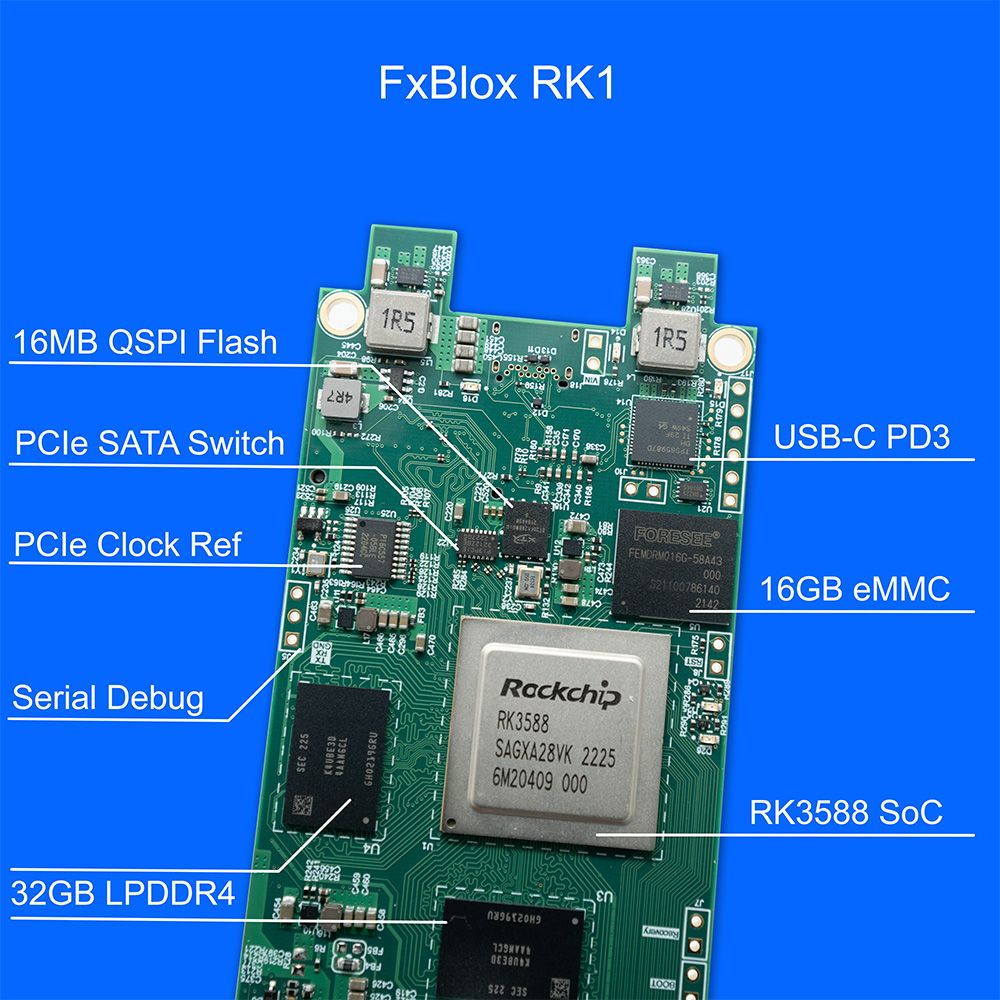
\includegraphics[width=\linewidth]{./assets/FxBlox_RK1.jpg} % Using path from prompt v2
    \captionof{figure}{\footnotesize Proven Hardware Execution: FxBlox RK1 SBC}
\end{center}
\vspace{1em}

\columnbreak % Move to next column

% --- Competitive Landscape ---
\subsection{Competitive Landscape}
\begin{center}
\resizebox{\linewidth}{!}{% Resize table to fit column width
\begin{tabular}{@{} l l l l l l @{}}
\toprule
\textbf{Company}     & \textbf{Openness} & \textbf{Modularity} & \textbf{Edge Focus} & \textbf{Ecosystem}   & \textbf{Role to Axior}        \\
\midrule
NVIDIA      & Closed   & Limited    & Partial    & Proprietary & Incumbent            \\
Google      & Closed   | Limited    & Partial    | Proprietary | Incumbent            \\
Apple       | Closed   | No         | Yes        | Proprietary | Incumbent            \\
Groq        | Closed   | No         | Cloud-only | Growing     | High-Perf Inference  \\
Tenstorrent | Partial  | Partial    | No         | Growing     | Training Innovator   \\
Flex Logix  | IP Vendor| N/A        | N/A        | IP Core Supplier | Technology Partner \\
\midrule % Separator for Axior
\textbf{Axior}       & \textbf{Open}     & \textbf{Full}       & \textbf{Full}       & \textbf{Open}        & \textbf{Inclusive \& Market Creator} \\
\bottomrule
\end{tabular}%
} % End resizebox
\end{center}
\vspace{0.5em}
\small The AI hardware market is dominated by closed, cloud-centric solutions from established giants (NVIDIA, Google, Apple), optimized for hyperscale data centers and proprietary ecosystems. New entrants like Tenstorrent are innovating in training acceleration, and Flex Logix provides valuable IP cores (which Axior leverages in our designs), but none address the critical gap in open, modular, edge-focused AI inference.
\vspace{0.3em}

\small Axior is not just competing; we are opening an entirely new segment: We empower advanced users, makers, and innovators, those who have been mere consumers, to become infrastructure providers themselves. This is a transformative shift, democratizing access to AI hardware and enabling a wave of user-driven innovation at the edge.

\vspace{1em}

% --- Team \& Execution Plan ---
\subsection{Team \& Execution Plan}
TransposeReal (Axior's parent company) is founded and led by Keyvan M. Sadeghi, a pioneer in AGI research and a proven hardware innovator.
\vspace{0.5em}
\begin{center}
\begin{tabular}{@{} l l p{0.5\linewidth} @{}}
\toprule
\textbf{Month} & \textbf{Milestone} & \textbf{Notes} \\
\midrule
1     & Lock IP deals, finalize floorplan \& TSMC NRE, Flex Logix \& Arm IP, DFT, EDA tools, backend engineering \\
2     & RTL handoff to backend, start SoM + carrier PCB layout & Fabrication, packaging, PCB layout, validation, test equipment \\
3     & Tape-out SoC, DVT board revision, software stack development & Linux BSP, NPU compiler, Hugging Face/vLLM, optimization, QA \\
4     & EVT board bring-up, OS bring-up, cluster validation & -- \\
5     & Beta hardware, compliance, developer kits & -- \\
6     & Production hardware, launch partners, open source toolchain & -- \\
\bottomrule
\end{tabular}
\end{center}

\vspace{1em}

% --- Industry Signals Box ---
\begin{infobox}[title=Industry Signals]
\scriptsize Placeholder for industry quotes, tweets, or news snippets validating the open AI hardware movement and edge inference demand. (See Community Momentum section for examples).
\end{infobox}

\end{multicols}


% ======================================================================
% PAGE 3: LATTICE, SOUL, VHYBZ DEEP DIVES & ROADMAP
% ======================================================================
\begin{center}
    {\brochuretitle\Huge\bfseries\color{axiorMagenta} Ecosystem Deep Dive \& Roadmap}
\end{center}
\vspace{1em}

\begin{multicols}{2}

% --- Lattice Deep Dive ---
\subsection{Lattice: Peer-to-Peer Agentic Mesh}
Lattice is an open protocol and runtime for mesh, agentic AI, enabling anyone, anywhere, to contribute compute and co-create resilient, intelligent systems beyond the limits of the cloud. Lattice is where anyone can help build, run, and own the next generation of AI infrastructure, powered by swarm intelligence, not centralized servers.
\vspace{0.5em}
\textbf{Features/Use Cases:}
\begin{itemize}[leftmargin=*, itemsep=0pt, topsep=2pt]
  \item \textbf{Agentic Nodes:} Every node is an autonomous agent, self-aware, self-optimizing, and capable of negotiating, executing, and verifying complex AI tasks.
  \item \textbf{Swarm Intelligence:} Intelligence emerges from real-time, peer-to-peer negotiation between nodes.
  \item \textbf{Heterogeneous by Design:} Unifies datacenter GPUs, edge devices, and home computers.
  \item \textbf{Use Cases:} Distributed LLM inference, federated learning, collaborative AI, mesh ETL, large-scale simulations, rendering farms.
\end{itemize}
\vspace{0.5em}
\begin{center}
    % Assuming lattice_diagram.png exists in ./assets/
    % \includegraphics[width=0.9\linewidth]{./assets/lattice_diagram.png} 
    \captionof{figure}{\footnotesize Lattice Mesh Protocol: Agentic nodes enable distributed workloads.}
    %\placeholder{lattice_diagram.png - Schematic of Lattice mesh protocol}
\end{center}
\vspace{1em}

% --- SOUL Deep Dive ---
\subsection{SOUL: Meta-Agent Framework}
SOUL is a modular, extensible Python framework for developing meta-agents, "Soulmades", characterized by inducing purposeful agency, distinct perspectives, and the ability to act based on an internal agenda into generic agents. It moves beyond reactive, text-wall generating models towards AI that exhibits "specific and objective" understanding.
\vspace{0.5em}
\textbf{Features/Key Concepts:}
\begin{itemize}[leftmargin=*, itemsep=0pt, topsep=2pt]
  \item Motivation Vector, Agenda, Perspective, Society of Minds.
  \item Modular, pluggable, supports multiple LLMs, knowledge sources, and governance.
  \item Features: Dynamic agenda, perspective-driven interaction, micro-agentic systems.
\end{itemize}
\vspace{0.5em}
\begin{center}
    % Assuming soul_architecture.png exists in ./assets/
    % \includegraphics[width=0.9\linewidth]{./assets/soul_architecture.png}
    \captionof{figure}{\footnotesize SOUL Framework: Modular architecture for agentic AI.}
    %\placeholder{soul_architecture.png - Block diagram of SOUL framework}
\end{center}
\vspace{1em}


% --- vhybZ Deep Dive ---
\subsection{vhybZ: Living Digital Experiences}
vhybZ is a new kind of platform where anyone can co-create dynamic, multimodal digital experiences alongside AI, going far beyond chatbot text walls or static apps. vhybZ is the next leap: we’re commoditizing Experience creation itself, supercharged by the latest advances in AI modality.
\vspace{0.5em}
\textbf{Features:}
\begin{itemize}[leftmargin=*, itemsep=0pt, topsep=2pt]
  \item \textbf{Experiences, not responses:} Time-based, interactive, and co-created.
  \item \textbf{Commons \& Remixability:} Every creation is a node in the Morphic Consensus Graph, attributed, remixable, and evolving.
  \item \textbf{Plug-and-play extensibility:} From LLMs to custom skills, vhybZ is modular by design.
  \item \textbf{Intuitive, not intimidating:} Craft, remix, and collaborate, no prompt engineering degree required.
\end{itemize}
\vspace{0.5em}
\begin{center}
    % Assuming vhybz_flow.png exists in ./assets/
    % \includegraphics[width=0.9\linewidth]{./assets/vhybz_flow.png}
    \captionof{figure}{\footnotesize vhybZ: Co-creating dynamic experiences with AI.}
    %\placeholder{vhybz_flow.png - Illustration of user/soulmade/memory interaction}
\end{center}
\vspace{1em}

\columnbreak % Move to next column for roadmap/tweets

% --- Community / Industry Momentum ---
\subsection{Community Momentum}
\begin{center}
\scriptsize
\begin{tabular}{ccc}
\begin{minipage}{0.22\linewidth}
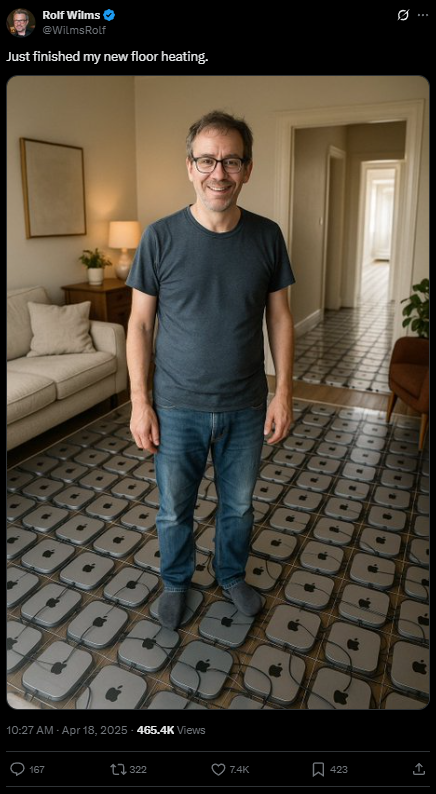
\includegraphics[width=\linewidth]{./assets/WilmsRolf.png}
\captionof{figure}{\scriptsize Rolf Wilms with Mac Mini floor}
\end{minipage} &
\begin{minipage}{0.22\linewidth}
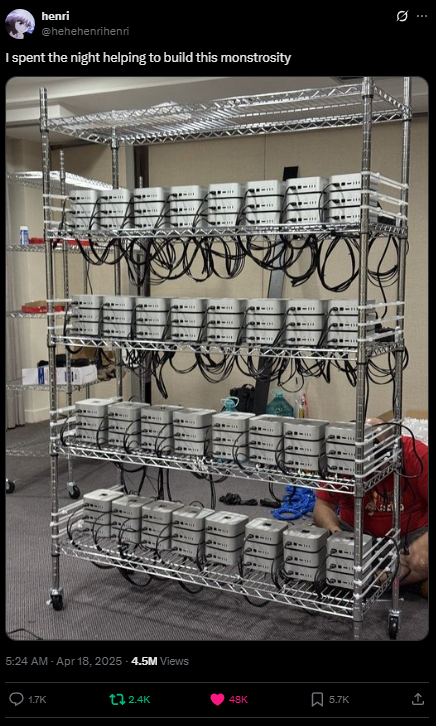
\includegraphics[width=\linewidth]{./assets/hehehenrihenri.png}
\captionof{figure}{\scriptsize Henri’s Mac Mini cluster rack}
\end{minipage} &
\begin{minipage}{0.22\linewidth}
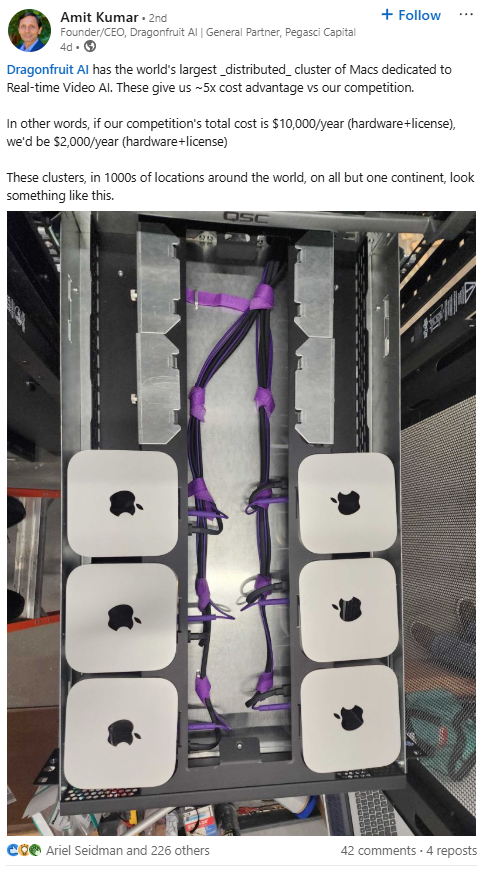
\includegraphics[width=\linewidth]{./assets/AmitKumar.png}
\captionof{figure}{\scriptsize Amit Kumar on distributed Mac clusters}
\end{minipage}
\end{tabular}
\end{center}

% --- Calls to Action / Sidebars ---
\begin{sidebar}[title=Join the Synthesis]
\footnotesize Connect with us, explore the open source codebases (coming soon), and help build the future of decentralized, agentic AI. Visit [Your Website Here] to learn more.
\end{sidebar}

\end{multicols} % End multicols before the full-width roadmap table

% ======================================================================
% SIX-MONTH PARALLEL ROADMAP (Full Width)
% ======================================================================
\vspace{1.5em}
\section{\color{axiorMagenta} Six-Month Parallel Roadmap}
\vspace{0.5em}

\begin{center}
\small % Use small font for the entire table
\begin{tabular}{@{} l p{0.18\textwidth} p{0.18\textwidth} p{0.2\textwidth} p{0.2\textwidth} @{}} % Adjusted widths to fit A4 page width
\toprule
\textbf{Month} & \textbf{Axior (Ai1) Hardware} & \textbf{Lattice (Mesh Protocol)} & \textbf{SOUL (Meta-Agent Framework)} & \textbf{vhybZ (Experience Platform)} \\
\midrule
\textbf{1} & Lock IP deals, finalize floorplan & Core protocol spec, node discovery, and MCP v0.1 & Core architecture refactor, Motivation/Agenda API, baseline LLM adapter & UX design sprint, core app skeleton, onboarding flow \\
\addlinespace % Add a little space between rows
\textbf{2} & RTL handoff to backend, start SoM + carrier PCB layout & Node profiling, peer-to-peer messaging, basic task allocation & Prompting engine, context assembler, first agentic demos & Experience engine MVP, chat/multimodal input, soulmade integration \\
\addlinespace
\textbf{3} & Tape-out SoC, DVT board revision, software stack development & Swarm allocation, GPU support, NAT traversal, monitoring & Society of Minds (multi-soulmade), governance hooks, evaluation/learning & Commons/remix backend, persistent memory layer, first user tests \\
\addlinespace
\textbf{4} & EVT board bring-up, OS bring-up, cluster validation & Robust fault-tolerance, mesh scaling, federated learning alpha & Knowledge adapters, advanced context, benchmarking & Mobile/web beta, extensibility plugins, collaborative Experiences \\
\addlinespace
\textbf{5} & Beta hardware, compliance, developer kits & Incentive layer, mesh storage, advanced monitoring & Performance optimization, developer docs, test suite & App store integration, user attribution, feedback loops \\
\addlinespace
\textbf{6} & Production hardware, launch partners, open source toolchain & v1.0 release: stable API, mesh incentives, partner onboarding & v1.0 release: refined agent model, core plugins, community examples & Public beta, creator tools, initial commons population \\
\bottomrule
\end{tabular}
\end{center}

\vfill % Push content up if there's extra space at the bottom

\end{document}
